\documentclass{presentation}

\title{Η Γνωριμία - Εφιάλτης ή Παράδεισος}
\subtitle{Γ Λυκείου}
\author[Λόλας]{Κωνσταντίνος Λόλας}
\institute[$10^ο$ ΓΕΛ]{$10^ο$ ΓΕΛ Θεσσαλονίκης}


\begin{document}

\begin{frame}
  \titlepage
\end{frame}

\begin{frame}{Το ταξίδι μας}
  \begin{figure}
    \centering
    \includegraphics[width=0.6 \textwidth]{"images/frodo"}
    \caption{Το ταξίδι ξεκινάει}
  \end{figure}
\end{frame}

\begin{frame}{Τελευταίος Χρόνος Σχολείο!}
  \begin{itemize}
    \item<1-> απολυτήριο ή εισαγωγικές?
    \item<2-> διάβασμα ή τουρίστας?
    \item<3-> έφηβος ή ενήλικας?
  \end{itemize}
\end{frame}

\begin{frame}{Πανελλαδικές 2022-2023}
  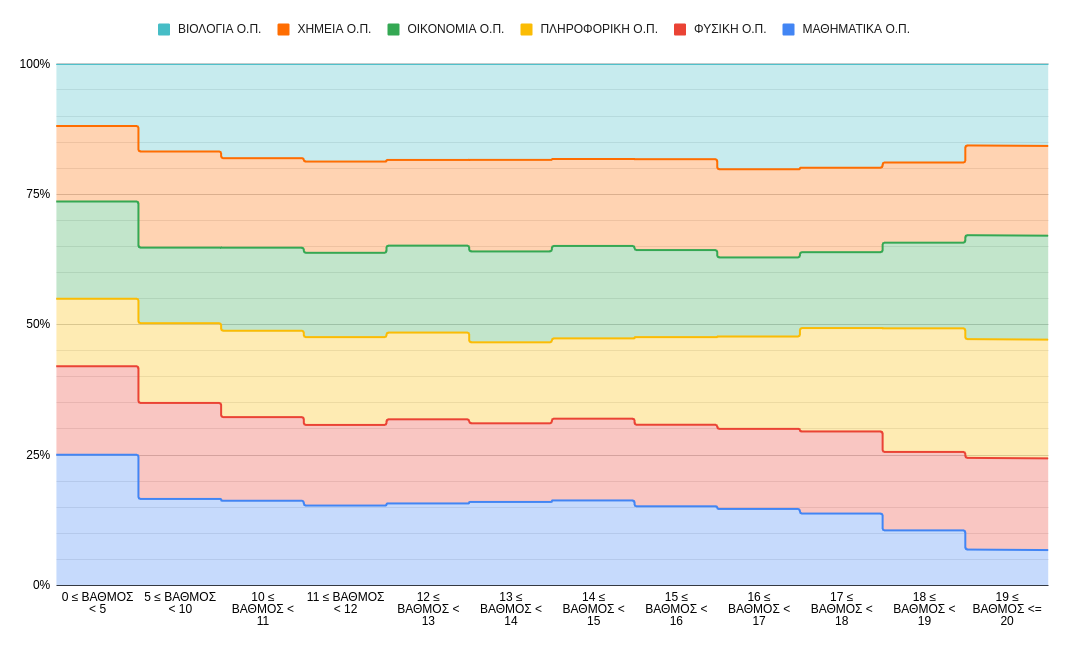
\includegraphics[width=\textwidth]{"images/Gnorimia.png"}
\end{frame}

\begin{frame}{Πανελλαδικές 2022-2023}
  \begin{figure}
    \centering
    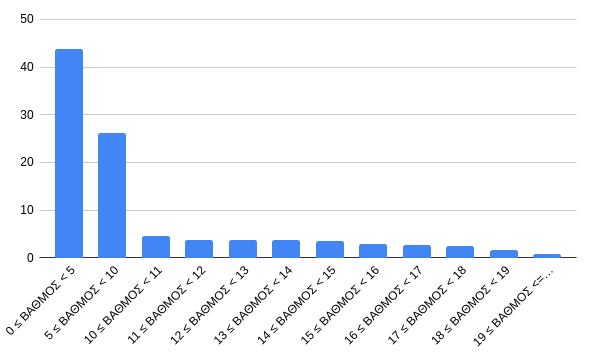
\includegraphics[width=0.48\textwidth]{"images/panelladikes22sop.png"}
    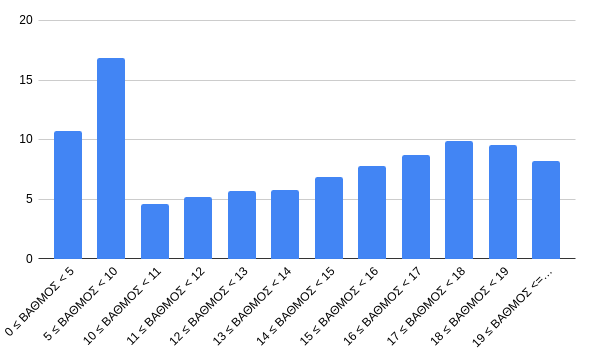
\includegraphics[width=0.48\textwidth]{"images/panelladikes22thet.png"}
    \caption{Αριστερά: ΣΟΠ, Δεξιά: Θετική}
  \end{figure}
\end{frame}

\begin{frame}{Πως θα βρεθούμε δεξιά?}
  \begin{itemize}
    \item Αποφασίστε ότι θα θυσιάσετε χρόνο \pause
    \item Μελετάμε και όχι διαβάζουμε ασκήσεις \pause
    \item Βοήθημα... δεν έχει καμία σημασία \pause
    \item Το σχολικό βιβλίο... Ευαγγέλιο!
  \end{itemize}
  \only<5>{και πάμε για το πιο παράξενο...}
\end{frame}

\begin{frame}{Φροντιστήριο - Ιδιαίτερα}
  \centering
  ΔΕΝ ΑΠΑΙΤΕΙΤΑΙ .-

  \only<2>{αν δεν σας έπεισα δείτε ξανά τα γραφήματα}
\end{frame}

\begin{frame}{Τάξη}
  \begin{itemize}
    \item Χαβαλές... φυσικά! \pause
    \item Καβγάς για την πιο ωραία λύση... επιβάλεται! \pause
    \item Ομιλίες μεταξύ σας... τι πιο ωραίο! \pause
    \item Αλλά επειδή απολαμβάνω ακόμα την δουλειά μου... την στιγμή του μαθήματος ΜΟΥΓΚΑ (εξήγηση)
  \end{itemize}
\end{frame}

\begin{frame}{Ο ρόλος του καθηγητή}
  \begin{itemize}
    \item απολαμβάνω το μάθημα \pause
    \item πρέπει να σας πείσω ότι μπορείτε \pause
    \item λύνω όλες τις απορίες ακόμα και μέσα από insta, messenger, moodle... \pause
    \item ασχολούμαι με όλους \pause
  \end{itemize}
  \only<5>{άρα εσείς απλά εκμεταλευτείτε το}
\end{frame}

\begin{frame}{Βαθμός}
  Στο Moodle υπάρχει ακριβώς ο τρόπος υπολογισμού του βαθμού σας που προκύπτει από:
  \begin{itemize}
    \item Ασκήσεις σχολικού
    \item Ασκήσεις Εξτρά
    \item Συμμετοχή (προφορικά τάξης)
    \item Διαγώνισμα - τεστ
    \item bonus
  \end{itemize}
  οπότε ξέρετε τον βαθμό σας ανά πάσα στιγμή!
\end{frame}

\begin{frame}{Ναι, αλλά τι θα μάθουμε}
  Όλα βρίσκονται στο moodle
  \begin{itemize}
    \item<1->Ανάλυση \pause
          \begin{enumerate}
            \item Συναρτήσεις - Ιδιότητες
                  \begin{enumerate}
                    \item Ορισμοί
                    \item Υπολογισμός Ορίων
                    \item Συνέχεια
                    \item Θεωρήματα Συνέχειας
                  \end{enumerate}
            \item Διαφορικός Λογισμός
                  \begin{enumerate}
                    \item Ορισμοί
                    \item Υπολογισμός παραγώγων
                    \item Θεωρήματα
                    \item Συνέπειες Θεωρημάτων
                    \item Μελέτη Συνάρτησης
                  \end{enumerate}
            \item Ολοκληρωτικός Λογισμός
                  \begin{enumerate}
                    \item Ορισμοί
                    \item Υπολογισμός ολοκληρωμάτων
                    \item Εμβαδά
                  \end{enumerate}
          \end{enumerate}
  \end{itemize}
\end{frame}

\begin{frame}{Θα έχουμε}
  \begin{figure}
    \centering
    \includegraphics[width=0.8\textwidth]{"images/difficulty"}
    \caption{Τα σκαμπανεβάσματα}
  \end{figure}
\end{frame}

\begin{frame}{Από πρότερες γνώσεις?}
  Παρατηρήσατε ότι η ύλη είναι μικρή? Άρα πού είναι η δυσκολία?
  \begin{itemize}
    \item Σύνολα
    \item Εξισώσεις
    \item Ανισώσεις \pause και το πιο σημαντικό \pause
    \item out of the box thinking
  \end{itemize}
\end{frame}

\begin{frame}{Θα έχουμε}
  \begin{figure}
    \centering
    \includegraphics[width=0.7\textwidth]{"images/weathertop"}
    \caption{Θεωρήματα Συνέχειας}
  \end{figure}
\end{frame}

\begin{frame}{Θα έχουμε}
  \begin{figure}
    \centering
    \includegraphics[width=0.9\textwidth]{"images/riverdale"}
    \caption{Παράγωγοι}
  \end{figure}
\end{frame}

\begin{frame}{Θα έχουμε}
  \begin{figure}
    \centering
    \includegraphics[width=0.3\textwidth]{"images/shelob"}
    \caption{Θεώρημα Rolle}
  \end{figure}
\end{frame}

\begin{frame}{Θα έχουμε}
  \begin{figure}
    \centering
    \includegraphics[width=0.6\textwidth]{"images/armyofdead"}
    \caption{Ολοκληρώματα}
  \end{figure}
\end{frame}

\begin{frame}{Και κάποτε...}
  \begin{figure}
    \centering
    \includegraphics[width=0.9\textwidth]{"images/frodo2"}
    \caption{Το ταξίδι τελειώνει}
  \end{figure}
\end{frame}

\begin{frame}
  Στο moodle θα βρίσκετε όλες τις παρουσιάσεις όπως και τις εργασίες που θα πρέπει να παραδίδετε.
\end{frame}

\end{document}
